\documentclass[11pt,a4paper]{article}
\usepackage[utf8]{inputenc}
\usepackage[T1]{fontenc}
\usepackage{amsthm} %numéroter les questions
\usepackage[english]{babel}
\usepackage{datetime}
\usepackage{xspace} % typographie IN
\usepackage{hyperref}% hyperliens
\usepackage[all]{hypcap} %lien pointe en haut des figures
\usepackage[french]{varioref} %voir x p y
\usepackage{fancyhdr}% en têtes
%\input cyracc.def
\usepackage[]{graphicx} %include pictures
\usepackage{pgfplots}
\usepackage[]{circuitikz}
\usepackage{ifthen}

\usepackage[top=1.3 in, bottom=1.3 in, left=1.3 in, right=1.3 in]{geometry} % Yeah, that's bad to play with margins
\usepackage[]{pdfpages}

\usepackage[]{attachfile}

\usepackage{float}
\usepackage{subfig}

\usepackage{todonotes} % \missingfigure
\usepackage{gensymb} % \ohm

\usepackage{framed}

\newdateformat{mydate}{v2.0.0}%hack pour remplacer \THEYEAR


\newboolean{corrige}
\ifx\correction\undefined
\setboolean{corrige}{false}% pas de corrigé
\else
\setboolean{corrige}{true}%corrigé
\fi

%\setboolean{corrige}{false}% pas de corrigé

\newboolean{annexes}
\setboolean{annexes}{true}%annexes
%\setboolean{annexes}{false}% pas de annexes

\definecolor{darkblue}{rgb}{0,0,0.5}

\newboolean{mos}
%\setboolean{mos}{true}%annexes
\setboolean{mos}{false}% pas de annexes

\usepackage{aeguill} %guillemets

%% fancy header & foot
\pagestyle{fancy}
%Numero du TP :
\def \labonumber {Project specifications}
\lhead{[ELEC-H-310] Choucroute numérique\\ \labonumber}
\rhead{\mydate\today\\ page \thepage}
\chead{\ifthenelse{\boolean{corrige}}{Corrigé}{}}
\cfoot{}
%%

\pdfinfo{
/Author (ULB -- BEAMS)
/Title (\labonumber ELEC-H-310)
/ModDate (D:\pdfdate)
}

\hypersetup{
pdftitle={\labonumber [ELEC-H-310] Choucroute numérique},
pdfauthor={ULB -- BEAMS},
pdfsubject={}
}

\theoremstyle{definition}% questions pas en italique
\newtheorem{Q}{Question}[] % numéroter les questions [section] ou non []

\newcommand{\reponse}[1]{% pour intégrer une réponse : \reponse{texte} : sera inclus si \boolean{corrige}
	\ifthenelse {\boolean{corrige}} {\paragraph{Réponse :} \color{darkblue}   #1\color{black}} {}
 }

\newcommand{\addcontentslinenono}[4]{\addtocontents{#1}{\protect\contentsline{#2}{#3}{#4}{}}}

\date{\vspace{-1.7cm}\mydate\today}
\title{\vspace{-2cm} \labonumber\\ Digital electronics [ELEC-H-310]\\Design of an automatic fanning system\ifthenelse{\boolean{corrige}}{~\\Corrigé}{}}

\setlength{\parskip}{0.2cm plus2mm minus1mm} %espacement entre §
\setlength{\parindent}{0pt}






%%%%%%%%%%%%%%%%%%%%%%%%%%%%%%%%%%%%%%%%%%%%%%%%%%%%%%%%%%%%%%%%%%%%%%%%%%%%%%%%%%%%%%%%%%%%%%%%%%%%%%%%%%%%%
%%%%%%%%%%%%%%%%%%%%%%%%%%%%%%%%%%%%%%%%%%%%%%%%%%%%%%%%%%%%%%%%%%%%%%%%%%%%%%%%%%%%%%%%%%%%%%%%%%%%%%%%%%%%%
%%%%%%%%%%%%%%%%%%%%%%%%%%%%%%%%%%%%%%%%%%%%%%%%%%%%%%%%%%%%%%%%%%%%%%%%%%%%%%%%%%%%%%%%%%%%%%%%%%%%%%%%%%%%%
% http://tex.stackexchange.com/questions/128123/circuitikz-current-source
% preparation to create bipoles

\makeatletter
\def\TikzBipolePath#1#2{\pgf@circ@bipole@path{#1}{#2}}

%\pgf@circ@Rlen = \pgfkeysvalueof{/tikz/circuitikz/bipoles/length}
\makeatother

\newlength{\ResUp} \newlength{\ResDown}
\newlength{\ResLeft} \newlength{\ResRight}

% set default dohicky size

\ctikzset{bipoles/doohicky/height/.initial=.4}
\ctikzset{bipoles/doohicky/width/.initial=.6}

% create doohicky shape

\pgfcircdeclarebipole{}
 {\ctikzvalof{bipoles/doohicky/height}}
 {doohicky}
 {\ctikzvalof{bipoles/doohicky/height}}
 {\ctikzvalof{bipoles/doohicky/width}}
 {
    \pgfsetlinewidth{\pgfkeysvalueof{/tikz/circuitikz/bipoles/thickness}\pgfstartlinewidth}
    \pgfextractx{\ResRight}{\northeast}
    \pgfextracty{\ResUp}{\northeast}
    \pgfextractx{\ResLeft}{\southwest}

  \pgfmoveto{\pgfpoint{\ResLeft}{0cm}}
    \pgfpathellipse{\pgfpoint{0.333\ResLeft}{0cm}}{\pgfpoint{0.667\ResRight}{0cm}}{\pgfpoint{0cm}{\ResUp}}
  \pgfmoveto{\pgfpoint{\ResRight}{0cm}}
    \pgfpathellipse{\pgfpoint{0.333\ResRight}{0cm}}{\pgfpoint{0.667\ResRight}{0cm}}{\pgfpoint{0cm}{\ResUp}}
  \pgfusepath{draw} %draw doohicky
    \pgfscope
    \pgfsetarrowsend{latex'}
    \pgfpathmoveto{\pgfpoint{0.667\ResLeft}{1.333\ResUp}}
    \pgfpathlineto{\pgfpoint{0.667\ResRight}{1.333\ResUp}}
    \pgfusepath{draw}   %draw arrow
    \endpgfscope
 }

% create doohicky to-path style

\def\doohickypath#1{\TikzBipolePath{doohicky}{#1}}
\tikzset{doohicky/.style = {\circuitikzbasekey, /tikz/to path=\doohickypath, l=#1}}

% end of setup
%%%%%%%%%%%%%%%%%%%%%%%%%%%%%%%%%%%%%%%%%%%%%%%%%%%%%%%%%%%%%%%%%%%%%%%%%%%%%%%%%%%%%%%%%%%%%%%%%%%%%%%%%%%%
%%%%%%%%%%%%%%%%%%%%%%%%%%%%%%%%%%%%%%%%%%%%%%%%%%%%%%%%%%%%%%%%%%%%%%%%%%%%%%%%%%%%%%%%%%%%%%%%%%%%%%%%%%%%
%%%%%%%%%%%%%%%%%%%%%%%%%%%%%%%%%%%%%%%%%%%%%%%%%%%%%%%%%%%%%%%%%%%%%%%%%%%%%%%%%%%%%%%%%%%%%%%%%%%%%%%%%%%%





















\begin{document}
\pagestyle{empty}
\maketitle
% \vspace*{-1cm}


% ########   ##      ##  ##########  ########     #####
%    ##      ###     ##      ##      ##     ##  ##     ##
%    ##      ## ##   ##      ##      ##     ##  ##     ##
%    ##      ##  ##  ##      ##      ########   ##     ##
%    ##      ##   ## ##      ##      ##   ##    ##     ##
%    ##      ##     ###      ##      ##    ##   ##     ##
% ########   ##      ##      ##      ##     ##    #####

\section{Introduction}
The aim of the project is to design a automatic fanning system for lazy teaching assistants. The fanning speed should be proportional to the illumination (and therefore to the heat) of the environment. 

\begin{center}
\begin{figure}[H]
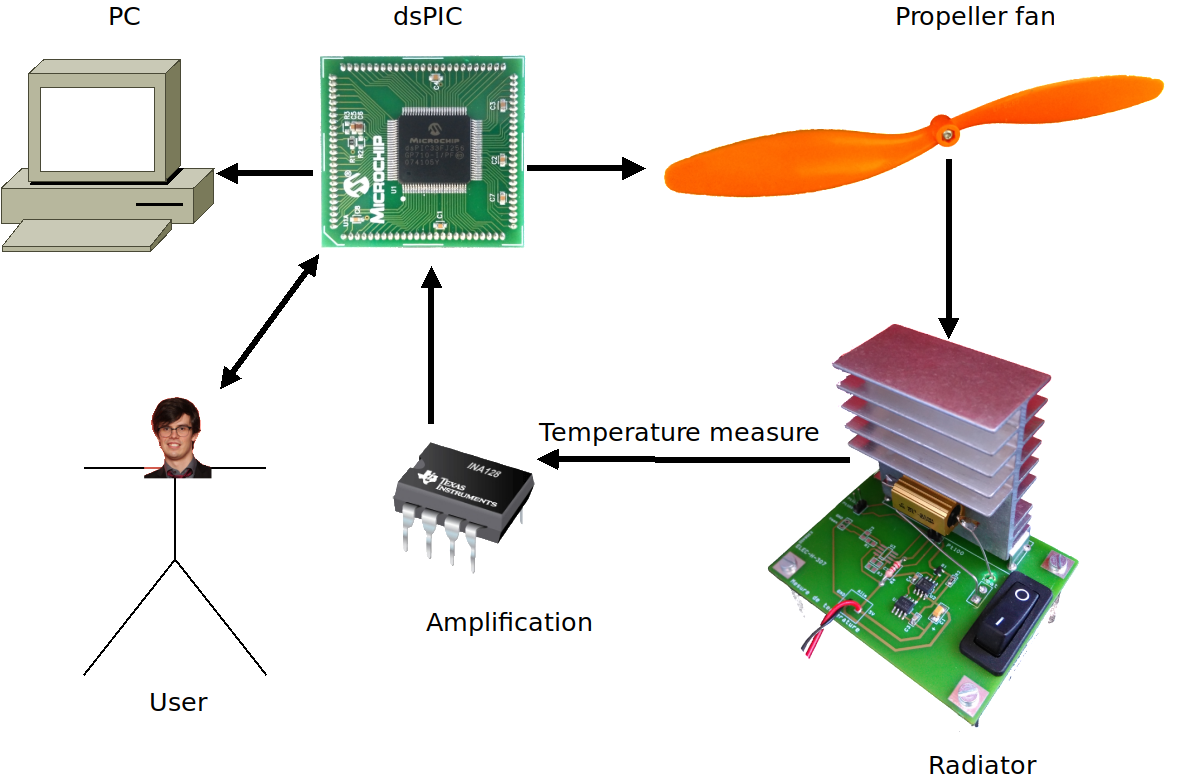
\includegraphics[width=\textwidth]{workflow}
\caption{Project diagram}
\label{fig:workflow}
\end{figure}
\end{center}

In this project, you will dispose of:
\begin{itemize}
	\item An PSOC board (CY8CKIT-059) with a custom ULB-designed extension board. 
	\item A propeller driven by a DC motor which will act as a fan. 
	\item A photoresistor (i.e. a light probe).
	\item A keyboard.
	\item A LCD screen (on the extension board).
	\item A serial connection with a computer making possible to prompt the temperature evolution through time.
\end{itemize}




%  #######      ###     ##     ##  ########   #########  ########
% ##     ##    ## ##    ##     ##     ##      ##         ##     ##
% ##          ##   ##   ##     ##     ##      ##         ##     ##
% ##         ##     ##  #########     ##      ######     ########
% ##         #########  ##     ##     ##      ##         ##   ##
% ##     ##  ##     ##  ##     ##     ##      ##         ##    ##
%  #######   ##     ##  ##     ##  ########   #########  ##     ##



\section{Project specifications}
The project is relatively complex, we will describe the requirements here.

The cooling of the teaching assistant is made by rotating the propeller at variable speed. 
You will need to control the power that will be delivered to the DC motor.

Similarly to the ELEC-H-301 labs, the power amplifier powering the motor is controlled by a PWM square wave (see section~\ref{sec:helice}).
Therefore, you will have to design a system to generate adjustable square waves.
The period of the square wave should be short compared with the mechanical time constant of the motor (its rotational speed should be almost constant during a PWM period).

By measuring the amount of light with the photoresistor, you will be able to design an open-loop regulation.
You may implement a very simple regulation procedure such as a proportional regulator. 

The luminous intensity is recorded with a photoresistor NSL-19M51 LDR. 
The value of the resistor $R$ vary with luminous intensity $I$ as follows: 
\begin{equation}
\frac{I}{I_0} = \left(\frac{R}{R_0}\right)^{-\gamma}
\end {equation}
where $R_0$ is the reference resistor value at luminous intensity $I_0$, and $\gamma$ is a characteristic of the photoresistor available in it's datasheet. Note that for our purposes, we can consider the illuminance to be proportional to the luminous intensity. Illuminance values vary from 1 to 10000 lux in our typical case (varying from pitch black to bright indoors)



The user must be able to operate the system by interacting with the keyboard and the LCD screen present on the expansion board.
Here are the operationnal commands:
\begin{itemize}
	\item Key `$\star$' + key `$\#$': the fanning mode is set to automatic, with a fanning speed proportional to illuminance.
	Example: ``$\star\#$" sets the fanning mode to automatic.
	\item One digit + key `$\#$': The fanning mode is set to manual, with a fanning speed proportional to the value entered (0 $\rightarrow$ fan is off, 9 $\rightarrow$ fan at maximum speed).
	Example: ``$4\#$" sets the fanning mode to manual, and the fanning speed to 4.
\end{itemize}

When no command is entered the screen should print the current voltage on the photoresistor: ``Vr=2.41V".
This screen should be refreshed every second.

Finally, the system will have to send the voltage on the photoresistor to the PC using the serial communication.
You will use the UART peripheral of the PSOC.
The voltage should be sent every second in the following format: ``2.41\textbackslash n".

We will use a simple serial communication software on the computer (such as Putty) to visualize the data. 






% ########   #########  #########  ##         #########  ##    ##   ########     #####    ##      ##
% ##     ##  ##         ##         ##         ##          ##  ##       ##      ##     ##  ###     ##
% ##     ##  ##         ##         ##         ##           ####        ##      ##     ##  ## ##   ##
% ########   ######     ######     ##         ######        ##         ##      ##     ##  ##  ##  ##
% ##   ##    ##         ##         ##         ##           ####        ##      ##     ##  ##   ## ##
% ##    ##   ##         ##         ##         ##          ##  ##       ##      ##     ##  ##     ###
% ##     ##  #########  ##         #########  #########  ##    ##   ########     #####    ##      ##


\section{Methodology}
Before starting such a project, you will have to think about the order of your actions.

It is strongly advised to start by reinterpreting the specifications in the form of a functional block diagram including the basic features of the project.
For each of these features, isolate the peripherals to use and make a schematic diagram of your algorithm.

Once done, implement the project block by block.
Start with a simple feature such as the command of the fan speed, then complete the rest of the project piece by piece.

Don't code anything too specific to a feature: remember that the different parts of your algorithm will have to interact with each others.
It might be beneficial to start by implementing the interfaces with the different blocks.
For instance, by coding a function that modify the fan speed.

The purpose behind this project is to program a system while understanding well what you are doing: no need to go too fast!



% ##       ##  #########   #######   ##     ##  ########   #########
% ###     ###  ##         ##     ##  ##     ##  ##     ##  ##
% ## ## ## ##  ##         ##         ##     ##  ##     ##  ##
% ##  ###  ##  ######      #######   ##     ##  ########   ######
% ##       ##  ##                ##  ##     ##  ##   ##    ##
% ##       ##  ##         ##     ##  ##     ##  ##    ##   ##
% ##       ##  #########   #######    #######   ##     ##  #########


\section{Luminous intensity measurement}

As mentioned above, the luminous intensity measurement is carried out by means of a photoresistance.
The electronic diagram is given in the figure~\ref{fig:meas-lum}.

\begin{figure}[H]
\center
	\begin{circuitikz}
				\draw
				(0,-2) to [phR=NSL-19M51, -o] (0,0)
				(0,-4) node [ground] {} to [R=$R_1$] (0,-2) 
				(0,0.5) node (vdd) {5V}
				(0,-2) to [short, -o] (1,-2) node (A) {}
				(0,-4) to [short, -o] (1,-4) node (B) {}
				(B) to[open, v=$V_{meas}$] (A)
				;
			\end{circuitikz}
\caption{Luminous intensity measurement with a NSL-19M51 photoresistor.}
\label{fig:meas-lum}
% \shorthandon{:!;}
\end{figure}

The photoresistor is mounted on a voltage divider. The (variable) photoresistor will determine the amount of current that flows through the two resistors, hence the voltage drop over resistor $R_1$. You should choose the value of $R_1$ such that the voltage drop over $R_1$ can be measured with the PSOC ADC for all possible values of the photoresistor. If you use a signle-ended ADC, don't forget to connect the ground of your circuit to the ground of your PSOC device. 





% ##     ##  #########  ##         ########    #######   #########
% ##     ##  ##         ##            ##      ##     ##  ##
% ##     ##  ##         ##            ##      ##         ##
% #########  ######     ##            ##      ##         ######
% ##     ##  ##         ##            ##      ##         ##
% ##     ##  ##         ##            ##      ##     ##  ##
% ##     ##  #########  #########  ########    #######   #########

\section{Power supply of the propeller}\label{sec:helice}
The PSOC doesn't supply enough power for the fan, a power circuit need to be added.
We will use a switching amplifier, those provide a square wave as output instead of a continuous signal.
Its schematics is illustrated on figure~\ref{fig:alim-moteur}.

% \missingfigure[figwidth=\textwidth]{Alimentation moteur}
\begin{figure}[H]
\center
% \shorthandoff{:!;}
\begin{circuitikz}
	\draw
	(1,0) node [nmos] (nmos1) {}%anchors are drain, source and gate.
	(1,1.5) node [pmos] (pmos1) {}% 1 = bottom pair
	(1,5) node [nmos] (nmos2) {}% 2 = top pair
	(1,6.5) node [pmos] (pmos2) {}
	(pmos2.source) node[above] () {5V}%Between parenthesis should be the label of the node. Don't any, here.
	(nmos2.source) node [ground] () {}
	(pmos1.source) node[above] () {5V}
	(nmos1.source) node[ground] () {}

	($(nmos2.drain)-(2,0)$) node [left]() {IN1} to [short, -*] +(1,0) node (A) {} -| (pmos2.gate)
	(A) -| (nmos2.gate)

	($(nmos1.drain)-(2,0)$) node [left]() {IN2} to [short, -*] +(1,0) node (B) {} -| (pmos1.gate)
	(B) -| (nmos1.gate)

	(pmos2.drain) to [short] +(3,0) to [twoport,t={Moteur}, bipoles/twoport/height=1.5] +(0,-4) |- (pmos1.drain)
	;
\end{circuitikz}
% \shorthandon{:!;}
\caption{Power supply of the motor.}
\label{fig:alim-moteur}
\end{figure}

Each branch of the converter can be seen as a MOS inverter: when the command is in high state, the bottom transistor is short-circuited while the top transistor is an open circuit.
The difference with classical logic circuit is that the transistors are able to provide higher currents.

The advantage of this system compared with a classical amplification is that it as a high efficiency.
As a first approximation, no power is dissipated in the switches, the power supply efficiency is close to 100\%.
An additional input named \textit{INHIB}, not represented on the figure, makes possible to deactivate the power supply.

The command of the power amplifier is made with square waves.
Several definitions associated with those waves are illustrated on figure~\ref{fig:square-wave}:
% \missingfigure[figwidth=\textwidth]{Figure onde carée avec temps de montée et de descente.}
\begin{figure}[H]
\center
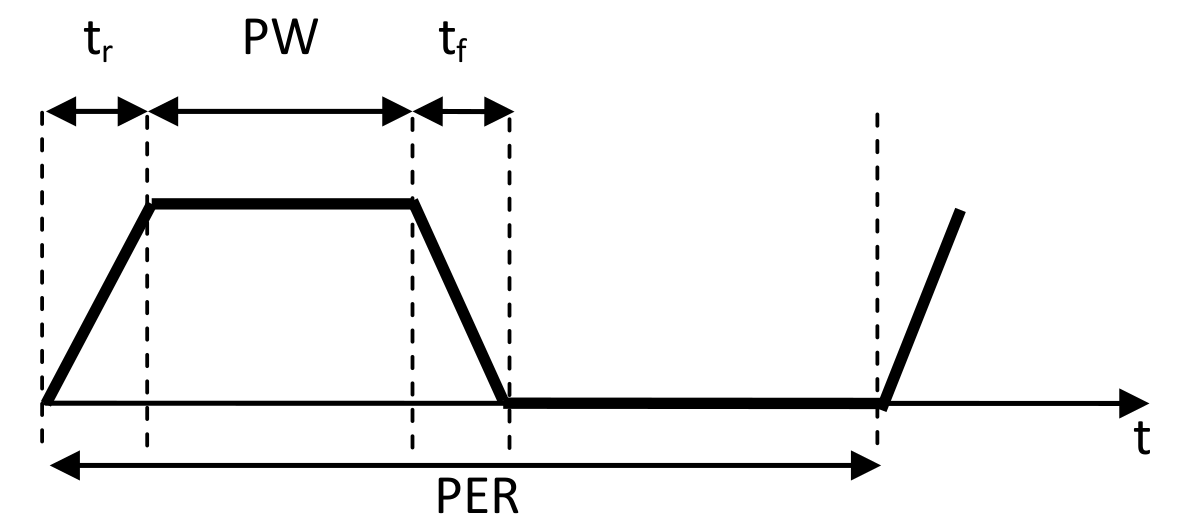
\includegraphics[width=0.6\textwidth]{square-wave}
\caption{Square wave.}
\label{fig:square-wave}
\end{figure}

The different characteristic times are as follows:
\begin{itemize}
	\item $PW$: Pulse Width, time in high state.
	\item $PER$: signal period.
	\item $t_r$: Rising time.
	\item $t_f$: Falling time.
\end{itemize}

In most cases, including this one, the rising and falling time are negligible.

An other characteristic is the duty cycle: it is defined as \[D = \frac{PW}{PER}\]
It is the proportion of time spent in high state during a period.

The PWM command (\textit{Pulse-Width Modulation}) consists of sending constant period square wave to the power circuit.
The mean value of the signal is proportional to the duty cycle.

In this case, the signal is the mean tension applied on the DC motor.
Let's take for instance the command signal provided by the PSOC on figure~\ref{fig:pwm}:
% \missingfigure[figwidth=\textwidth]{PWM}
\begin{figure}[H]
\center
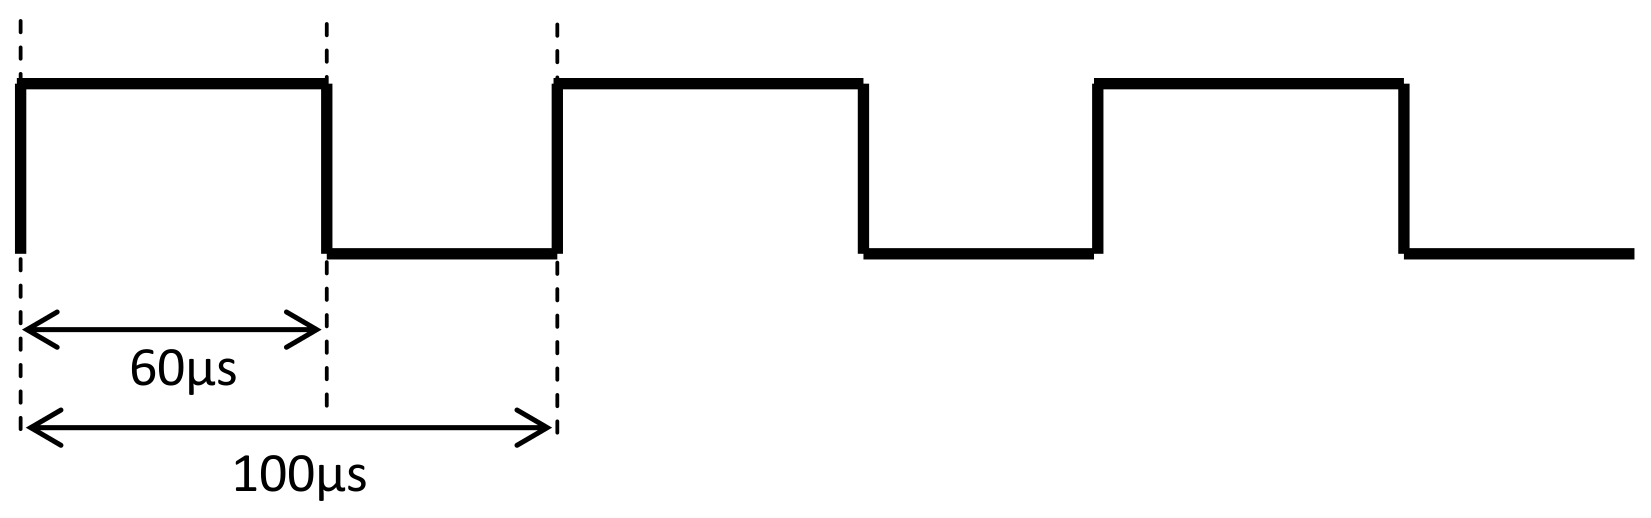
\includegraphics[width=0.7\textwidth]{pwm}
\caption{PWM Signal with a duty cycle of 60~\%.}
\label{fig:pwm}
\end{figure}

This signal is applied on the pin \texttt{IN1} of the motor and pin \texttt{IN2} is connected the ground.

The period is $100 \mu s$ and the duty cycle is $60\%$.
When the command is in high state, V- is at 0~V and the converter imposes a voltage of 5~V to the motor.
When it is not the case, the voltage is 0~V.
The mean voltage is then $0.6 \cdot 5V  = 3 V$.

\begin{framed}
By playing with the duty cycle, you will be able to modify the propeller speed.
The duty cycle is then the control variable of your regulator.
\end{framed}

The PSOC has a peripheral to generated PWM waves: you need to define its period then to configure a specific register to enter the duty cycle.



\end{document}
